
\chapter{Image analysis} 
 
Creation of sensing machines working in the environment necessitate 
a validation of in the context of physical scenarios. Some of these 
scenario are flooding, insect clouds, pollutions, fires.

The focus of this chapter are tools and methods allowing to produce inputs
for physical  simulations. These simulations are compute intensive. It is expected
that they could be achieved using discrete computation models such as
cellular automata. It is expected that they will cooperate with network simulations
in various ways: production of stimuli on sensors, or dangers for the sensor network
itself.

The interest of image anlysis is to produce regions that share similar characteristics.
Analysis follows a conventional flow, starting from a picture coming from sources such as
photographies, maps, radar images, to obtain regions of interests, on which physical simultaion will
take place.

An example of processing on such regions has been deveopped with cellular automata
reproducing fire expansions on region havaing some vegetations (shown Figure \ref{fig:AhmedFire},
movie demonstration and report \cite{AhmedFire}).


\begin{figure}[hbtp]
\begin{center} 
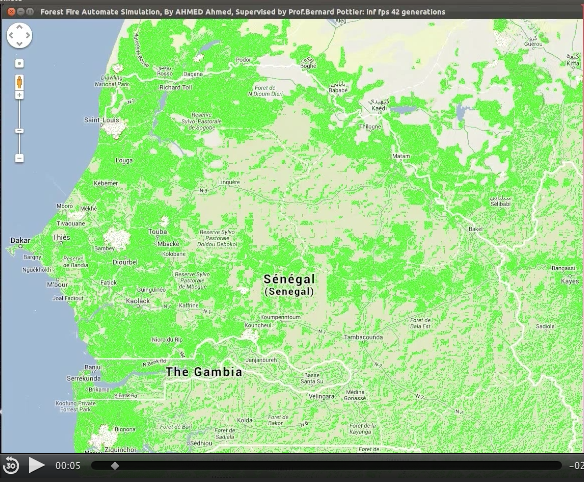
\includegraphics[width=10cm]{AhmedFire.png}
\caption{Fire simulation (or locust expansion) using Cellular Automata implementing  states such as:
vegetation, burning, ashes.}
\label{fig:AhmedFire}
\end{center}
\end{figure}

\section{General flow}

\begin{figure}[hbtp]
\begin{center} 
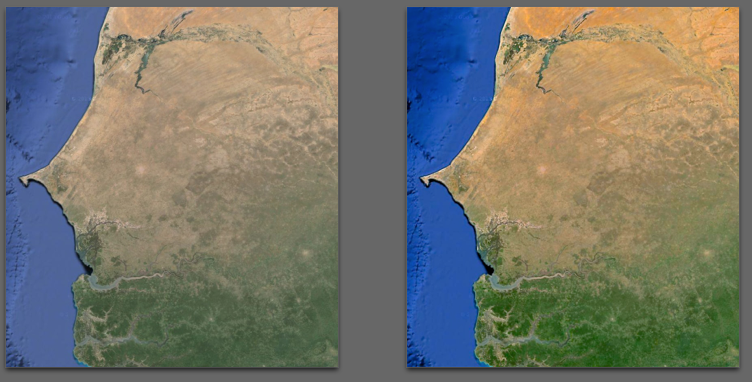
\includegraphics[width=10cm]{SenegalSideBySide.png}
\caption{Modifying original image for better contrasts or coulour selections}
\label{fig:sideBySide}
\end{center}
\end{figure}
  
